\documentclass[a4paper,11pt]{article}
%\documentclass[a4paper,9pt,landscape]{article}
\usepackage[english]{babel}
%\usepackage[utf8]{inputenc}
\usepackage{graphicx}
\usepackage{fullpage}
\usepackage{amsmath}
\usepackage{pdfpages}
\usepackage{listings}
\usepackage{color}
\usepackage{multicol}
\usepackage{fancyhdr}
\usepackage[top=1.5cm, bottom=4cm, left=2.5cm, right=2.5cm]{geometry}
\usepackage{hyperref}
\usepackage{verbatim}
\setlength{\voffset}{-9pt}
%\setlength{\hoffset}{-1in}
%\setlength{\marginparsep}{0.5cm}


\setlength{\parindent}{1cm}
%\setlength{\parskip}{-0.1cm}
%\setlength{\columnseprule}{0.4pt}
\setlength{\footskip}{0.5cm}
\setlength{\headheight}{15pt}
\setlength{\headsep}{2cm}

\fancypagestyle{tcr}{%
  \fancyhf{} %clear all headers and footers fields
  \fancyhead[R]{\thepage}
  \fancyhead[L]{\textbf{Lab No 2 TDDC78}}
  \renewcommand{\headrulewidth}{0.4pt}
}

\definecolor{dkgreen}{rgb}{0,0.6,0}
\definecolor{gray}{rgb}{0.5,0.5,0.5}
\definecolor{mauve}{rgb}{0.58,0,0.82}
\lstset{
  title=\lstname,
  frame=t,
  %aboveskip=-0.5cm, 
  %belowskip=0pt,
  basicstyle=\footnotesize\ttfamily,
  keywordstyle=\color{blue},          % keyword style
  commentstyle=\color{dkgreen},       % comment style
  stringstyle=\color{mauve},         % string literal style
  showstringspaces=false,         % underline spaces within strings
  tabsize=2,
  language=C,
  title=\caption,
  %xleftmargin=-1cm
}


\begin{document}
%% title stuff
\title{Lab No 2 TDDC78}
\author{Linus Mellberg (linme560) \and Oskar Aagaard (oskaa489)}
\date{\today}
\maketitle
\pagebreak
%\setcounter{page}{1}
%\begin{multicols}{2}
\thispagestyle{tcr}
\pagestyle{tcr}
%\tableofcontents

\section{Averaging filter}
The averaging filter works by convoluting the input image with a gaussian filter kernel.
This will do a weighted average on the pixel and the pixels surrounding it.
Since the gaussian kernel is symmetric the the calculation can be simplified, this makes the problem linear in the radius of the kernel.
\subsection{Description of the program}
The filtering program developed during this laboration task uses the library pthread to do parallelization of the filtering program.
The filtering is split into two phases.
First the filtering along the x-axis is done and after that the filtering along the y-axis.
If the output from each phase is transposed these two phases become equal.
This should also make data accesses more local, there is no need to scan along the y-axis of a buffer.
Only the writes of single output pixels are done along the y-axis.

The picture is split into equal regions along the y-axis.
Each thread is then given a region that it filters.
The operation that is done in each phase is to apply the filter along the x-axis (calculate a weighted sum for every pixel).
The output from this operation is written to a new buffer and it is also transposed by switching x and y coordinates.
After the first phase is done a join of the threads is needed, as this phase needs to be finished before the next one starts.
When all threads have finished new regions are calculated along the x-axis.
The threads are then started again but with the transposed output buffer as input.
The output is written back to the first input buffer.
When all threads have finished the filtered image is written to disk.

\subsection{Result and graphs}

If a small filter kernel is used the read and write operations becomes a large part of the execution time of the program.
This is a sequencial operation that might be possibly to optimize, but this is left out of this report.
This has made us ignore the time used for reading and writing to disk from of the execution time calculations used below.

As with the MPI implementation this programs performs in the expected way. 
The execution time is proportional to the radius of the filter kernel and to the number of pixels in the image.
It is inversely proportional to the number of processes.
A difference between the two implementation is that this implementation seems to perform better on very small problem sizes.
The linear performance also hold on small problem sizes.
This is probably casued by the fact that there is very little overhead.
The only thing that has to be done is the initialization of the threads, this seems to be fast.

Figure \ref{16_threads_runtime} shows the execution time when running the program with 16 threads.
The linear behaviour in the radius can clearly be seen.
There is a constant offset that seems to be slightly larger for larger images.
It is not certain what the reason for this is, but for example it might be becuause of cache effects.

In figure \ref{im4} the performance on the largest image is shown.
The execution time here is also proportional to the radius of the filter kernel.
The inversely propotional dependence on the number of threads can also be seen.

When both the complexity and number of processes are changed the result is figure \ref{complexity}.
The three lines should correspond to different problem size but with the number of processes changed to compensate for this.
The larger images are a bit slower than the smaller ones, but asymptotically they seem to behave in the same way.
The difference might have many reason and one of them might again be cache effects.
The small images might fit better into the cache.

The number of floating points operations per second was also estimated.
This number should ideally be the same for all problem sizes on a fixed number of processes, it should also be proportional to the number of processesa.
This is not true for small problem sizes, but for larger problem sizes the FLOP per process count converges to a certain value.
The FLOP per process for small problem sizes seems to be about half of the value for large problem sizes.
Again there can be many reasons for this. Again for example cache effects or overhead.
For the bigger problem sizes the MFLOP count converges to about 2000 MFLOP per process.

\begin{figure}[!h]
  \caption{Run times related to radius on 16 threads for the different images.}
  \label{16_threads_runtime}
  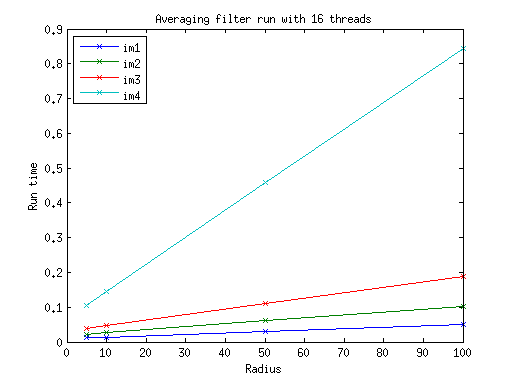
\includegraphics[scale=0.9]{../plots/16_threads_runtime_radius.png}
\end{figure}
\begin{figure}[!h]
  \caption{Run times for different numbers of cores on im4.ppm.}
  \label{im4}
  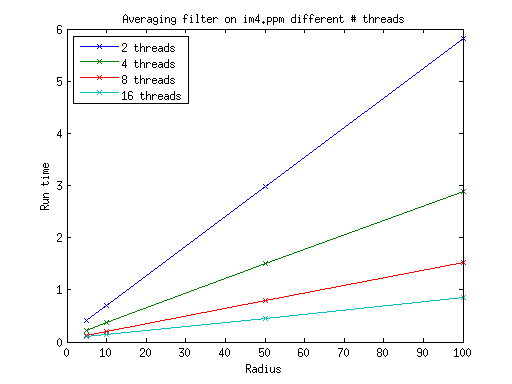
\includegraphics[scale=0.9]{../plots/im4_pthread_runtime_radius.png}
\end{figure}
\begin{figure}[!h]
  \caption{Run times related to radius when increasing image size and number of cores.}
  \label{complexity}
  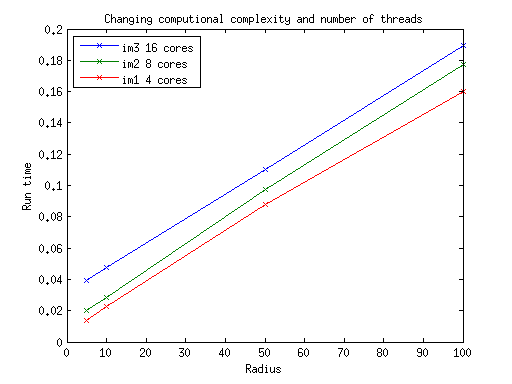
\includegraphics[scale=0.9]{../plots/pthread_compexity_and_no_processes.png}
\end{figure}

\clearpage

\section{Thresholding filter}
The thresholding filter turns a coloured image into a black and white image. A pixel in the filtered image is black if its colour intensity is lower than a threshold, otherwise white. The colour intensity is calculated by summing the RGB values of a pixel. The threshold is determined by the average colour intensity of all the pixels.
\subsection{Description of the program}
The first step is determining the average pixel intensity by adding the RGB values of each pixel in the image together and dividing by the total number of pixels. The program then looks at the RGB sum for each pixel in turn and determines if the corresponding pixel of the output image should be black or white by whether it's greater or lower than the average.

\paragraph\noindent\textbf{Overview of the linear program}
\begin{itemize}
\renewcommand{\labelitemi}{$\bullet$}
\item Load image from disk
\item Calculate average RGB sum
\item Calculate output image
\item Write image to disk
\end{itemize}

Because there is no dependency between pixels during either of the two calculations the work can easily be divided between an arbitrary amount of processors by giving them an as equal share as possible with no concern for locality. 

The program calculates the work share of each processor and then creates structs containing this information for each individual processor. The threads are then started and the processors then calculate the RGB sum of their share and the total sum is then calculated by each process adding their sum to a shared variable using a mutex lock to ensure correctness. The threads are then joined and created again for the second calculation and then finally joined again at the end.

\paragraph\noindent\textbf{Overview of the parallel program}

\begin{itemize}
\renewcommand{\labelitemi}{$\bullet$}
\item Load image from disk on root processor
\item Calculate work shares
\item Start new threads to calculate average RGB sum in parallel
\item Sum the results into a global variable.
\item Start new threads to Calculate output image in parallel
\item Wait for threads to finish
\item Root process writes image to disk
\end{itemize}

\subsection{Result and graphs}
Using pthreads which can share memory a big improvement over the mpi implementation is expected. As we can see in figure \ref{thresc_123} and \ref{thresc_4} this is also the case. We have beautiful scaling that is nearly linear in the amount of processors when the problem size is big and gradually less so for smaller input. For \emph{im1.ppm} the work load is so small that it seems not to be worth threading, but when the run time is less than a millisecond it is hard to tell.

The run time is also nearly linear in problem size for sufficiently large problems which means that run times when both problem size and thread count is proportionally increased are almost the same. We see some straight lines on the y-axis of figure \ref{thresc_123} that show this.

\begin{figure}[!h]
  \caption{Run times related to number of cores for images 1, 2 and 3}
  \label{thresc_123}
  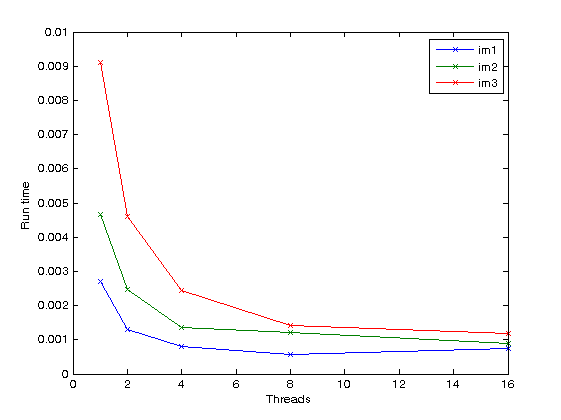
\includegraphics[scale=0.9]{../plots/pthread_im123.png}
\end{figure}
\begin{figure}[!h]
  \caption{Run times related to number of cores for image 4.}
  \label{thresc_4}
  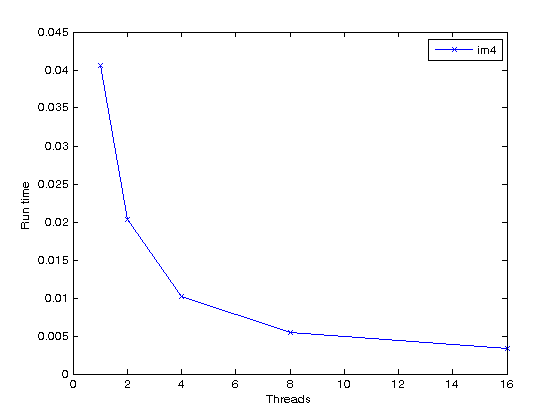
\includegraphics[scale=0.9]{../plots/pthread_im4.png}
\end{figure}

\begin{table}[h!]
  \label{mpixelspersecond}
  \caption{$MPixels/Second$ when running with different amount of threads and on different data.}
  \begin{tabular}[h]{|l|l|l|l|l|l|}
    \hline
                  & 1     & 2     & 4     & 8     & 16\\
    \hline
    im1           & 135.41 & 183.31 & 184.94 & 68.89  & 21.77\\ 
    im2           & 150.01 & 209.17 & 274.71 & 201.65 & 63.15\\ 
    im3           & 146.25 & 209.72 & 274.44 & 275.62 & 138.23\\ 
    im4           & 145.07 & 212.56 & 286.41 & 332.90 & 297.42\\
    \hline
  \end{tabular}
\end{table}

\begin{comment}
\cite{fenwick}
\clearpage
\begin{thebibliography}{9}
  \bibitem{fenwick}
    Binary Indexed Trees,
    \emph{Algortihmist}.\\
    \url{http://community.topcoder.com/tc?module=Static\&d1=tutorials\&d2=binaryIndexedTrees}
  \bibitem{ppm}
    Mark Nelson,
    \emph{Arithmetic Coding + Statistical Modeling = Data Compression}, 1991.\\
    \url{http://marknelson.us/1991/02/01/arithmetic-coding-statistical-modeling-data-compression/}
  \bibitem{ppmc}
    PPM
    \url{http://www.cs.ucf.edu/courses/cap5015/ppm.pdf}

\end{thebibliography}a
\end{comment}

\clearpage
\section{Source code}
Files that are included but not listed here were downloaded from the course webpage and not modified.

\lstinputlisting[caption=blurmain.c]{../blurmain.c}
\clearpage
\lstinputlisting[caption=blurfilter.c]{../blurfilter.c}
\clearpage
\lstinputlisting[caption=blurfilter.c]{../blurfilter.h}
\end{document}
